%
%  Introduction
% ==============
%

\chapter{Introduction}
\label{Ch:Intro}

The Advanced Wakefield Experiment (AWAKE)~\cite{awake_collaboration:2014}, located at the old CNGS\footnote{The CERN Neutrinos to Gran Sasso (CNGS) experiment was operational between 2006 and 2012.} facility at CERN, became operational in December 2016.
It is a proof-of-concept Proton Driven Plasma Wakefield Accelerator (PDPWFA) using a proton bunch from the Super Proton Synchrotron (SPS) as its drive bunch.

AWAKE is currently in Run~1, where the interaction between the proton drive bunch and the plasma will be studied, and where a long electron witness bunch will be injected to sample the wakefields.
Run~2 is planned to start after the next Long Shutdown of the LHC~\cite{bernardini:2016} scheduled for 2019 and 2020, when significant upgrades will also be made to AWAKE.
Run~2 will attempt to accelerate a short, intense electron bunch to high energy, while avoiding growth in emittance and large energy spread.
In preparation for Run~2, a number of design choices needs to be made based on the results of Run~1 as well as simulations of Run~2.
The work presented in this thesis primarily focuses on the beam loading of a short electron witness bunch through simulations, in preparation for AWAKE Run~2.

The key results are presented in Publication~\ref{Pub:BL17}, with the studies leading up to this publication presented in two conference papers: Publication~\ref{Pub:IPAC15} and~\ref{Pub:NAPAC16}.
A third conference paper, Publication~\ref{Pub:IPAC17}, covers the integration of the AWAKE experiment with the CERN control system, which is the main contribution to Run~1 in this PhD project.

In this chapter we will first cover some of the key concepts involved in plasma wakefield acceleration techniques relevant to the work presented in this thesis.
The design of the AWAKE experiment itself is laid out in more detail in the next chapter, and the integration of the AWAKE experiment into the CERN Control System is described in the third chapter.
The fourth and fifth chapters outlines the simulation works, which makes up most of the thesis work.

% ================================================================================================================================ %
%  Plasma Wakefield Acceleration
% ================================================================================================================================ %
\section{Plasma Wakefield Acceleration}
\label{Int:PWFA}

Accelerating particle bunches in a plasma is an attractive concept as plasmas are capable of sustaining significantly higher accelerating fields than RF structures used in conventional accelerators can.
Such RF structures suffer electrical breakdowns at very high electric fields, and these breakdowns can over time damage the structures~\cite{braun:2003}.
This puts an upper limit on the accelerating gradient.
These breakdowns cause damage to the surfaces of the RF cavities.
In practice, the upper limit is determined by the statistical probability of a breakdown and the acceptable number of breakdowns in a given period of time~\cite{pritzkau:2002}, and the practical limit is therefore lower -- around $100\unit{MV/m}$~\cite{aicheler:2012}.

While RF cavities use standing electromagnetic waves to accelerate particles, plasma accelerators use an energetic bunch to drive strong electromagnetic wakefields in the plasma.
The two main techniques for producing these strong accelerating fields are by the use of an intense laser beam, or by the use of a particle drive bunch.
Laser accelerator techniques were investigated in the early 1970s~\cite{chan:1971, palmer:1972}, and wakefield acceleration techniques through the use of computer simulations at the end of the decade~\cite{tajima:1979}.
Using particle bunches to drive accelerating wakefields were proposed some time later, in 1985~\cite{chen:1985}.

Both the particle bunch and laser driver techniques utilise a neutral plasma where the collective motion of the free electrons define the main parameters of the accelerating structure.
The characteristic time of the electron motion is related to the plasma frequency, $\omega_{pe}$, and the characteristic length is related to the plasma wavelength, $\lambda_{pe}$.
\begin{equation}
    \lambda_{pe} = \frac{2\pi c}{\omega_{pe}}, \quad
    \omega_{pe}  = \sqrt{\frac{n_{0}e^{2}}{m_{e}\epsilon_{0}}}, \label{EQ:PWFA:L0W0}
\end{equation}
where $n_{0}$ is the initial plasma electron density, $e$ is the elementary charge, $m_{e}$ is the electron mass, and $\epsilon_{0}$ is the vacuum permittivity~\cite{tonks:1929, esarey:1996, pecseli:2012}.
Here we ignore the ion mass and we assume the plasma is cold, i.e. we ignore the thermal motion of the electrons.
The characteristic time and length of ion motion scales as the square root of the mass difference compared to the plasma electrons and tend, depending on the ion mass, to be a few orders of magnitude longer than those of the electrons.
In the case of very long accelerating structures, the motion of the ions may become an issue~\cite{rosenzweig:2005}.

Plasmas can, in general, sustain accelerating electric fields on the order of the non-relativistic wave-breaking field~\cite{dawson:1959, esarey:1996}
\begin{equation}
    E_{\mathrm{WB}} = \frac{m_{e} c \omega_{pe}}{e}. \label{EQ:EWB}
\end{equation}
For instance, for a plasma density of $10^{18}\unit{cm}^{-3}$, the maximum field is on the order of $100\unit{GV/m}$.
This has been inferred by experiment in the mid 1990s when a few electrons were accelerated to over $40\unit{MeV}$ in about $300\unit{\mu m}$ of Helium plasma driven by a $25\unit{TW}$ pico second laser~\cite{modena:1995}.

Both techniques require a drive bunch that deposits energy into the plasma in the form of wakefields.
The drive bunch is trailed by another bunch, called the \textit{witness bunch}, which draws energy from the fields in order to accelerate.
We thus see a transfer of energy from the drive bunch to the witness bunch through plasma as the intermediate medium~\cite{muggli:2009}.
Let us briefly introduce the core principle of the two methods of plasma wakefield acceleration. 

% ================================================================================================================================ %
\subsection{Laser Driven Acceleration}
\label{Int:LWFA}

In a laser wakefield driven plasma accelerator (LWFA), the plasma acts like a transformer, changing high frequency transverse field of the laser pulse into a low frequency longitudinal wave~\cite{malka:2009}.
The effect driving the accelerating fields was described by Tajima and Dawson in 1979, and can be summarised as follows:
The ponderomotive force at the front of the laser pulse drives plasma electrons forward, while at the back of the pulse it pushes them backwards.
This generates a longitudinal wave that is at its most efficient when the length of the laser pulse $L_{ph} = \lambda_{pe}/2$~\cite{tajima:1979}.
A trailing particle bunch can then be position at the accelerating flank of the field.
In some instances plasma electrons can also be captured and accelerated instead.

% ================================================================================================================================ %
\subsection{Beam Driven Acceleration}
\label{Int:BDPWFA}

In a beam or bunch driven plasma wakefield acceleration (BDPWFA or just PWFA) a drive bunch of charged particles is sent through a section of neutral plasma.
The space charge of the drive bunch displaces the plasma electrons, which oscillate at the plasma frequency, creating periodic regions of low and high electron density generating strong wakefields.
The longitudinal and transverse fields generated by this wake are then loaded by a trailing beam of particles.
The principles behind this technique were formulated in the 1980s by Pisin Chen \etal~\cite{chen:1985}.

Any type of charged particle bunch can be used in such an accelerator.
Most experiments to date have used electrons.
It has been shown that energy can be transferred from one or more electron drive bunch to a single electron witness bunch, or trailing electrons in an electron drive bunch, in multiple past experiments~\cite{rosenzweig:1988, blumenfeld:2007, kallos:2007, litos:2014, nakajima:1990}.
In one such experiment, at the Stanford Linear Accelerator Center (SLAC), a $42\unit{GeV}$ electron beam passing through an $85\unit{cm}$ section of ionised Lithium vapour saw the trailing part of the electron bunch reach $85\unit{GeV}$.
This corresponds to a gradient of $52\unit{GV/m}$~\cite{blumenfeld:2007}.

A limitation using an electron bunch with a similar initial charge and energy for both drive and witness bunches is that the witness bunch will rapidly gain energy, while the drive bunch loses energy, leading to dephasing.
This both causes the drive bunch to quickly decelerate, while the witness bunch undergoing acceleration will at the same time catch up with the drive bunch.
Typically propagation length of an electron drive bunch is a few tens of centimetres of plasma due to limited energy in the bunch.

% ================================================================================================================================ %
%  Beam and Plasma Interactions
% ================================================================================================================================ %
\section{Bunch and Plasma Interactions}
\label{Int:BPI}

As a relativistic, charged bunch propagates through plasma, it affects the local density of the plasma electrons.
The charged bunch generates strong transverse fields, pushing or pulling the plasma electrons away or towards the propagation axis of the beam~\cite{lee:2001,adli:2016b}.
As the heavier plasma ions will move on a much longer time scale, due to inertia, the plasma electrons expelled from the axis will be pulled back towards it by the ion charge.
The electrons will tend to overshoot the axis, creating an oscillation system.
A positively charged drive bunch will initially pull the electrons towards the axis, where they overshoot, creating a similar effect to a negative drive bunch, but with a half-period phase offset.
The oscillation period is determined by the plasma frequency of the electrons~\cite{hogan:2016,muggli:2017}. 

\begin{figure}[hbt]
    \centering
    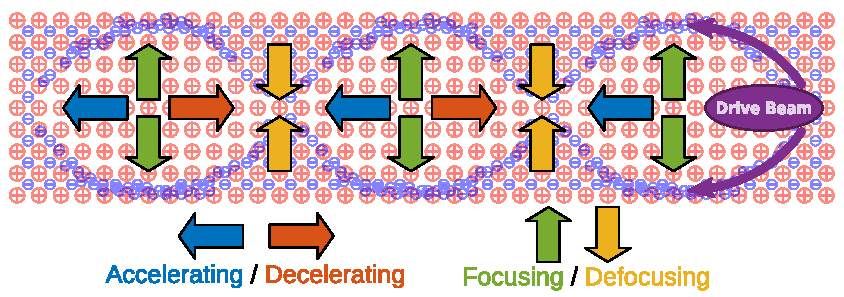
\includegraphics[width=0.85\linewidth]{figures/PlasmaWakefield}
    \caption{\label{Fig:PWFA:Illust} Illustration of a plasma wakefield accelerating structure with a single electron drive bunch.
    The drive bunch produces a series of focusing\slash de\-fo\-cus\-ing and accelerating\slash de\-cel\-e\-rat\-ing regions, as seen for an electron witness bunch.}
\end{figure}

A conceptual illustration of an electron bunch driven plasma accelerator is shown in Figure~\ref{Fig:PWFA:Illust}.
Several regions of decreasing magnitude of accelerating\slash decelerating and focusing\slash defocusing are generated behind the drive bunch.
By positioning a trailing beam in an optimal phase, such a bunch can be both accelerated and focused.
The drive bunch needs to be shorter than the plasma period for this structure to be most effective, but multiple short drive bunches with a separation of the plasma wavelength can resonantly amplify the wakefields.

% ================================================================================================================================ %
\subsection{Emittance and Twiss Parameters}
\label{Int:BPI:EnTwiss}

Before we continue, let us briefly introduce an important set of parameter when describing the evolution of a charged particle bunch or beam: the beam emittance, and the Twiss parameters also known as the Courant-Snyder parameters~\cite{courant:1958}.
The Twiss parameters are useful quantities to describe the trajectory of particles in an accelerator in the transverse phase space.
The following, brief, derivation is based on Klauss Wille, \textit{The Physics of Particle Accelerators}~\cite{wille:2001}.

The general solution to the trajectory of particles in an accelerator is given by
\begin{align}
    x(s)          &=  \sqrt{\epsilon\beta(s)} \cos\left[\Psi(s) + \phi\right] \label{EQ:PTrajX} \\
    x^{\prime}(s) &= -\sqrt{\frac{\epsilon}{\beta(s)}}
                     \left[\alpha(s)\cos\left(\Psi(s) + \phi\right) + \sin\left(\Psi(s) + \phi\right)\right], \label{EQ:PTrajXP}
\end{align}
where the parameter
\begin{equation}
    \alpha(s) \equiv -\frac{\beta^{\prime}(s)}{2}. \label{EQ:TwissAlpha}
\end{equation}

In order to arrive at an expression describing the particle motion in the $x-x^\prime$ plane, we must eliminate the terms depending on $\Psi$.
We thus obtain:
\begin{equation}
    \epsilon = \frac{x^2}{\beta(s)} + \left(\frac{\alpha(s)}{\sqrt{\beta(s)}}x + \sqrt{\beta(s)}x^{\prime}\right)^2.
\end{equation}

By introducing the parameter
\begin{equation}
    \gamma(s) \equiv \frac{1+\alpha^2(s)}{\beta(s)}, \label{EQ:TwissGamma}
\end{equation}
we obtain
\begin{equation}
    \epsilon^2 = \gamma(s)x^2(s) + 2\alpha(s)x(s)x^{\prime}(s) + \beta(s)x^{\prime 2}(s). \label{EQ:EmittFull}
\end{equation}

\begin{figure}[hbt]
    \centering
    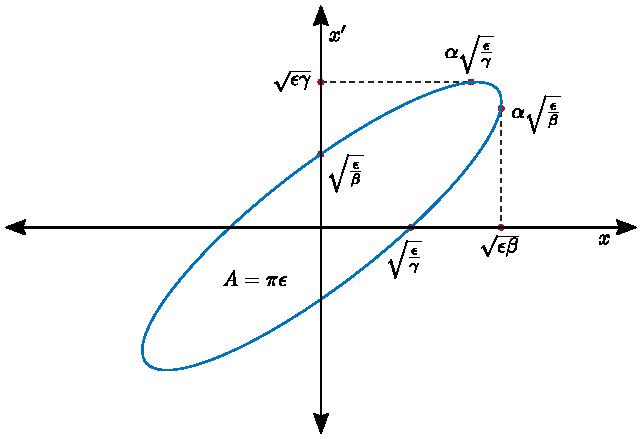
\includegraphics[width=0.8\linewidth]{figures/Twiss}
    \caption{\label{Fig:BPI:Twiss}
        The phase space ellipse of bunch particles.
        The figure is recreated from Figure~3.23 by Klauss Wille in \textit{The Physics of Particle Accelerators}~\cite{wille:2001}.
    }
\end{figure}

This equation describes an ellipse in phase space, and how the Twiss parameters $\alpha$, $\beta$ and $\gamma$ relates to the geometric emittance $\epsilon$ and the shape of the ellipse is illustrated in Figure~\ref{Fig:BPI:Twiss}.
It is often useful to refer to normalised emittance, which is the geometric emittance multiplied with the relativistic factor
\begin{equation}
    \emitN = \epsilon \gammar. \label{EQ:NormEmit}
\end{equation}
Normalised emittance stays constant during acceleration, while geometric emittance does not.

% ================================================================================================================================ %
\subsection{The Drive Bunch}
\label{Int:BPI:Drive}

The wakefields generated by a charged drive bunch are given by the Lorentz force
\begin{equation}
    \vec{W} = \frac{\vec{F}}{q_{b}} = \vec{E} + \vec{v}_{b} \times \vec{B}, \label{EQ:Lorentz}
\end{equation}
where $q_{b}$ is the bunch charge and $\vec{v}_{b}$ is the bunch velocity.
We define the longitudinal coordinate in the frame of the bunch along its direction of propagation as
\begin{equation}
    \xi \equiv z - v_{b}t \approx z - ct, \label{EQ:Xi}
\end{equation}
and for the purpose of the following derivations, we use a cylindrical coordinate system $(r, \xi)$.
It follows, then, that the longitudinal wakefield is only determined by the longitudinal component of the electric field -- to the first order -- such that
\begin{equation}
    W_{\parallel}(r,\xi) = E_{z}(r,\xi). \label{EQ:Wz}
\end{equation}
The transverse wakefield, on the other hand, also depends on the magnetic field such that
\begin{equation}
    W_{\perp}(r,\xi) = E_{r}(r,\xi) - cB_{\theta}(r,\xi), \label{EQ:Wr}
\end{equation}
where we again take the velocity of the bunch to be $v_{b} \approx c$.

A charged bunch will diverge and lengthen due to space charge, but since the bunch is relativistic the effect is of no significance over a few metres of plasma.
In the transverse plane, however, the bunch is subject to the Lorentz force given by the transverse component of Equation~\ref{EQ:Lorentz}.
Taking Maxwell's equations and $B_{\theta} = v_{b}E_{r}/c^{2}$~\cite{schindl:1999}, the strength can be estimated using an infinitely long, uniform bunch of density $n_{b}$:
\begin{equation}
    F_{\perp} = q_{b}(E_{r} - v_{b}B_{\theta})
              = q_{b}E_{r}\left(1 - \frac{v_{b}^{2}}{c^{2}}\right)
              = \frac{1}{\gamma^2}q_{b}E_{r}. \label{EQ:DeFocR}
\end{equation}
The implication of this is that for relativistic bunches, the transverse dynamics are dominated by emittance and external forces.
Dephasing is a potential concern in long plasma sections:
However, at high energies, the distance $\Delta L$ between two particles of a bunch does not change significantly over a distance $L$.
The change can be estimated as
\begin{equation}
    \frac{\Delta L}{L} \approx \frac{1}{\gamma^{2}}\frac{\Delta\gamma}{\gamma} \label{EQ:DePhL}
\end{equation}
for two sample particles with energy difference $\Delta\gamma$~\cite{muggli:2017}.

% ================================================================================================================================ %
\subsection{The Transformer Ratio}
\label{Int:BPI:TRat}

The aim of plasma wakefield acceleration is to transfer energy from a drive bunch to a witness bunch via the plasma.

Following Ruth \etal~\cite{ruth:1985}, let us consider a drive bunch of zero length, with $N_{d}$ particles of individual energy $E_{d}$, and $W_{e}(\xi)$ is the wakefield per unit charge.
The energy loss of the bunch in the decelerating field is given by:
\begin{equation}
    \frac{\deriv (N_{d}E_{d})}{\deriv z} = - N_{d}^{2}e^{2}W_{e}(0), \label{EQ:TRat:Drive}
\end{equation}
where $\xi_{d} = 0$ is the position of the drive bunch.

The trailing witness bunch at position $\xi_{w}$, will see the wakefield left by the drive bunch as well as its own wakefield:
\begin{equation}
    \frac{\deriv (N_{w}E_{w})}{\deriv z}
        = - N_{w}^{2}e^{2}W_{e}(0) - N_{d}N_{w}e^{2}W_{e}(\xi_{w}), \label{EQ:TRat:Witness}
\end{equation}
where $N_{w}$ is the number of particles in the witness bunch, and $E_{w}$ is their individual energy.

As required by energy conservation, the total energy of the system cannot increase.
It thus follows that
\begin{equation}
    (N_{d}^{2} + N_{w}^{2})W_{e}(0) + N_{d}N_{w}W_{e}(\xi_{w}) \geq 0, \label{EQ:TRat:EConv}
\end{equation}
giving the requirement that the acceleration gradient experienced by a trailing particle satisfies
\begin{equation}
    \frac{\deriv E_{w}}{\deriv z} \leq (2N_{d} - N_{w})e^{2}W_{e}(0). \label{EQ:TRat:Grad}
\end{equation}

Assuming the drive bunch transfers all of its energy to the wakefields, it would stop after a distance
\begin{equation}
    L = \frac{E_{d}}{N_{d}e^{2}W_{e}(0)}. \label{EQ:Trat:LStop}
\end{equation}
The energy a witness bunch particle can gain must satisfy
\begin{equation}
    \Delta E_{w} = \frac{\deriv E_{w}}{\deriv z}L
                 \leq E_{d}\left(2-\frac{N_{w}}{N_{d}}\right). \label{EQ:TRat:DeltaE}
\end{equation}

The maximum energy gain approaches twice the energy of the drive bunch as $N_{w} \to 0$.
In a wakefield accelerator we define the maximum accelerating field \textit{behind} the drive bunch where the witness beam is position, to the maximum decelerating field \textit{within} the drive bunch as the \textit{transformer ratio}~\cite{muggli:2017}
\begin{equation}
    R = \frac{E_{+}}{E_{-}}. \label{EQ:TRat}
\end{equation}
While the maximum transformer ratio is $2$, larger values can be achieved by for instance bunch ramping~\cite{bane:1985} or by a train of bunches~\cite{jing:2006}.

To maximise efficiency in the transfer of energy from the drive bunch to the plasma, the bunch should have a length $k_{pe}\sigma_{z} \simeq \sqrt{2}$~\cite{lu:2005,lee:2000}.
Its transverse size should also stay within $k_{pe}\sigma_{r} \lesssim 1$ as wider bunches will cause filamentation instabilities~\cite{allen:2012,sentoku:2003}.

% ================================================================================================================================ %
\subsection{Plasma Regimes}
\label{Int:BPI:Reg}

The effect of a bunch on the plasma, as it travels through it, can be divided into a linear and a non-linear regime.
In addition to these two there is a transitional region between these often referred to as the \textit{quasi-linear} regime.
It is also useful in some contexts to distinguish between a non-linear and a highly non-linear regime.
Figure~\ref{Fig:BPI:Regime} illustrates the four regimes considered here, with representative proton drive bunches.

\begin{figure}[hbt]
    \centering
    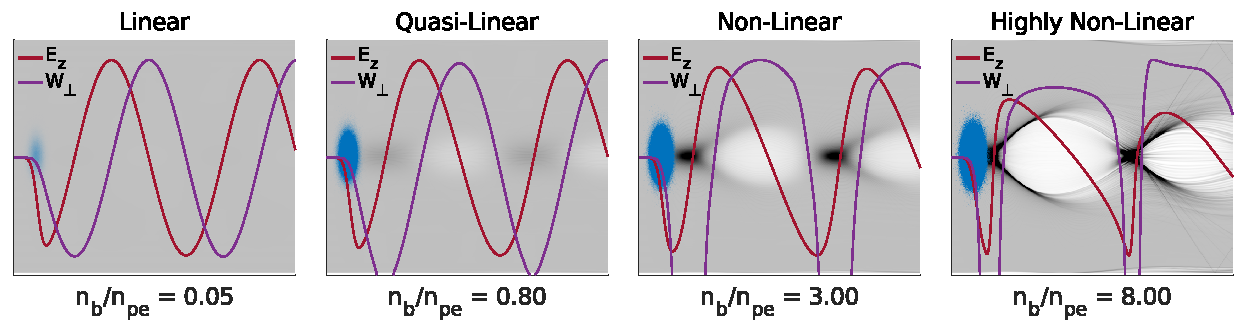
\includegraphics[width=1.0\linewidth]{figures/Regimes}
    \caption{\label{Fig:BPI:Regime}
        Four sample simulations of a proton bunch of varying density $n_{b}$ with respect to the plasma density $n_{pe}$.
        Each simulation is representative for the four regimes.
        The longitudinal and perpendicular wakefields are normalised to their own maxima to illustrate their shape rather than their absolute magnitude.
    }
\end{figure}

% ================================================================================================================================ %
\subsubsection{The Linear Regime}
\label{Int:BPI:Lin}

When the charge density of the bunch is smaller than that of the plasma, $n_{b} \ll n_{pe}$ (see Figure~\ref{Fig:BPI:Regime}), the system is in the \textit{linear regime}.
The linear regime is not of much interest for accelerator applications as it does not utilise the full potential of the plasma for generating strong wakefields, and the transverse and longitudinal fields have local variations in the are where we want to accelerate a witness bunch.
These variations will strongly affect the bunch energy spread and emittance.
However, this regime is interesting from a theoretical perspective because it is well described analytically~\cite{muggli:2017}.

A linear theory for plasma accelerators can be derived using a cold, non-relativistic fluid model of the plasma.
The response of the cold plasma can be found from the linearised equations of motion and continuity, and the Maxwell equations. (For examples of linearisation, see~\cite{pecseli:2012,chen:1974}.)
The equations of motion and continuity are linearised assuming the perturbed plasma density $n_{1}$ is much smaller than the unperturbed density $n_{0} = n_{pe}$~\cite{chen:1987}.
By further combining the fluid equation and the Poisson equation~\cite{katsouleas:1987}, a wave equation for for the plasma density perturbation by the bunch can be derived~\cite{chen:1987,muggli:2017}:
\begin{equation}
    \frac{\partial^{2}}{\partial\xi^{2}}n_{1} + k_{pe}^{2}n_{1} = \frac{q_{b}}{e}k_{pe}^{2}n_{b}, \label{EQ:BeamPlasmaWF}
\end{equation}
where we still assume $n_{b} \ll n_{pe}$.

The solution to Equation~\ref{EQ:BeamPlasmaWF} in the longitudinal dimension is the Green’s function for a harmonic oscillator in one dimension~\cite{katsouleas:1987}, and the radial dependency can be calculated from two-dimensional theory for different radial profiles~\cite{chen:1987}.
For a bunch with a Gaussian profile in both dimensions, the wakefields are
\begin{align}
    W_{\parallel}(r,\xi) &= \frac{e}{\epsilon_{0}}
        \int_{-\infty}^{\xi} n_{b\parallel}(\xi^{\prime}) \cos\left[k_{pe}(\xi-\xi^{\prime})\right] \,\deriv\xi^{\prime} \,\cdot\, R(r) \label{EQ:WzFull} \\
    W_{\perp}(r,\xi) &= \frac{e}{\epsilon_{0}k_{pe}}
        \int_{-\infty}^{\xi} n_{b\parallel}(\xi^{\prime}) \sin\left[k_{pe}(\xi-\xi^{\prime})\right] \,\deriv\xi^{\prime} \,\cdot\, \frac{\mathrm{d}}{\mathrm{d}r}R(r), \label{EQ:WrFull}
\end{align}
where the transverse dependency $R(r)$ is
\begin{align}
    R(r) &= k_{pe}^{2} \int_{0}^{r} n_{b\perp}(r^{\prime}) I_{0}(k_{pe}r^{\prime})
           K_{0}(k_{pe}r) \,r^{\prime}\,\deriv r^{\prime} \nonumber \\
         &+ k_{pe}^{2} \int_{r}^{\infty} n_{b\perp}(r^{\prime}) I_{0}(k_{pe}r)
           K_{0}(k_{pe}r^{\prime}) \,r^{\prime}\,\deriv r^{\prime}. \label{EQ:WFRadial}
\end{align}
Here $I_{0}$ and $K_{0}$ are the zeroth-order modified Bessel functions of the first and second kind, respectively~\cite{chen:1987,muggli:2017}.

\begin{figure}[hbt]
    \centering
    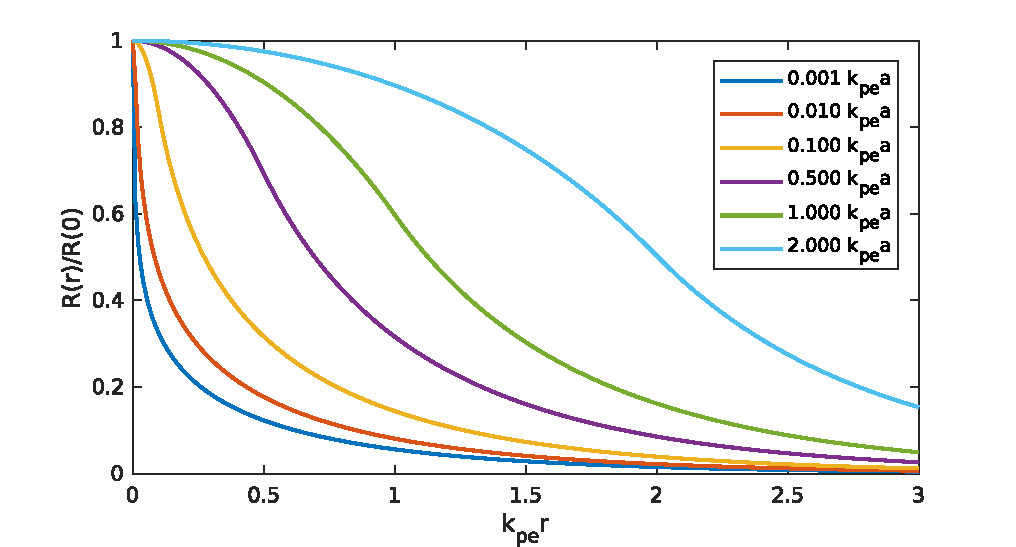
\includegraphics[width=0.8125\linewidth,trim={0mm 0mm 0mm 0mm},clip]{figures/RepKatsouleas1987}
    \caption{\label{Fig:BPI:Kat87}
        The radial function $R(r)$ for a range of uniform bunches, cut off at a radius $a$, up to twice the plasma skin depth $k_{pe}^{-1}$.
        The plot is reproduced from Katsouleas \etal~\cite{katsouleas:1987}.
    }
\end{figure}

As can be seen from Figure~\ref{Fig:BPI:Kat87}, the longitudinal wakefield is at its maximum on-axis.
For very wide bunches, $\sigma_{r} \gg k_{pe}^{-1}$, we converge at the one-dimensional result.
For very narrow bunches, $\sigma_{r} \ll k_{pe}^{-1}$, the maximum decreases rapidly with radius causing different parts of the witness bunch at different radii to see different accelerating fields.
The cosine component of Equation~\ref{EQ:WzFull} also implies longitudinal variations of the accelerating field.
Combined, these produce a large energy spread for the accelerating bunch of finite extent $\sigma_r, \sigma_z$.
Additionally, the radially varying focusing field from Equation~\ref{EQ:WrFull} produces emittance growth~\cite{muggli:2017,katsouleas:1987}.

% ================================================================================================================================ %
\subsubsection{The Non-Linear Regime}
\label{Int:BPI:NLin}

When the beam density $n_{b} > n_{pe}$, the system enters the non-linear regime, and becomes highly non-linear when $n_{b} \gg n_{pe}$ -- often referred to as the \textit{blowout regime} (see Figure~\ref{Fig:BPI:Regime}).
In this regime the plasma electrons are expelled entirely from the region around the axis, to form a region populated by only plasma ions.
As the ions are practically stationary on the time scale of the plasma electrons, they form a uniform column of positive charge.
The electrons displaced by the space charge of the drive bunch are pulled back on axis by the ions in the form a thin sheath with the shape of a bubble.
Hence, this regime is also sometimes referred to as the \textit{bubble regime}.
The large transverse forces produced by the drive bunch in this regime, followed by the strong restoring force of the ion channel, produces a large plasma electron density spike behind the formed bubble~\cite{dawson:1959,rosenzweig:1991}.
Using this regime for plasma wakefield acceleration was proposed by Rosenzweig \etal ~in 1991~\cite{rosenzweig:1991}.

\begin{figure}[hbt]
    \centering
    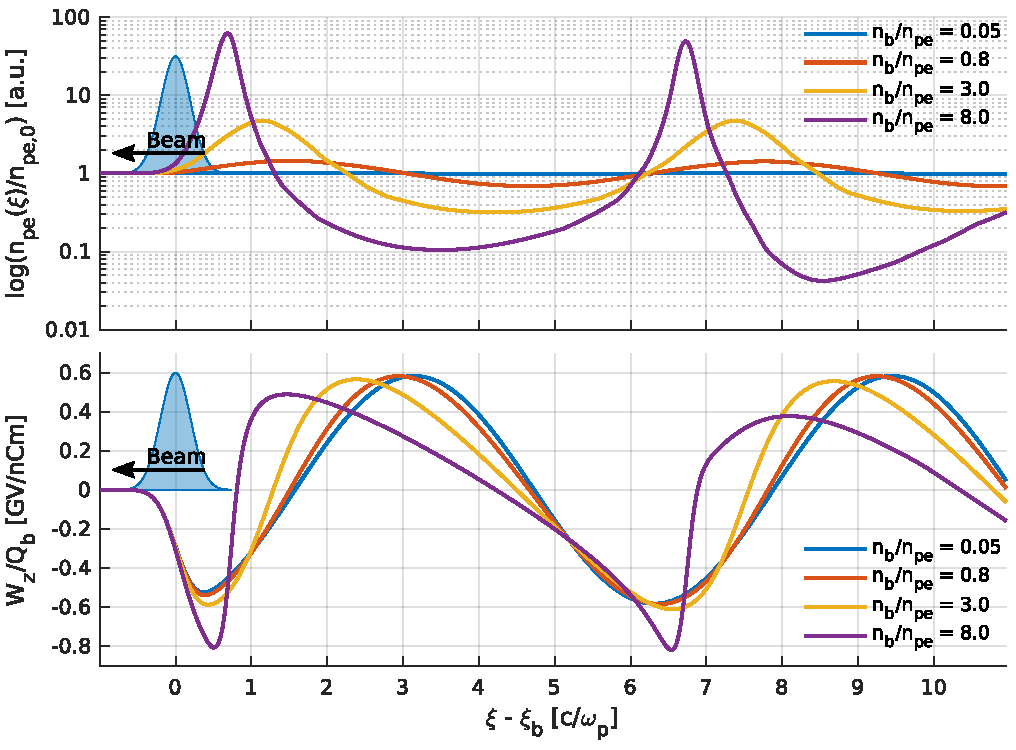
\includegraphics[width=0.875\linewidth,trim={0mm 0mm 0mm 0mm},clip]{figures/Density}
    \caption{\label{Fig:BPI:Density}
        \textbf{Top:} Relative on-axis plasma density perturbation for a $n_{b}/n_{pe}$ density ratio corresponding to a linear, quasi-linear, non-linear and highly non-linear case.
        \textbf{Bottom:} Longitudinal wakefield per unit of beam charge for the same four cases.
        The four samples correspond to the four cases presented in Figure~\ref{Fig:BPI:Regime}.
    }
\end{figure}

The radial wakefield, $W_{r}$, varies linear linearly with radius, while the accelerating wakefield, $W_{z}$, is uniform within the bubble.
In other words: while the focusing by the radial wakefield prevents emittance growth, the longitudinal wakefield preserves the energy spread of a bunch slice -- both advantages over the linear regime.

Unlike in the linear regime, there is no full theory describing the non-linear regime.
However, a non-linear kinetic theory has been developed by Lu \etal ~that is valid under certain assumed conditions~\cite{lu:2006a,lu:2006}.

The magnitude of the plasma electron perturbation and the relative strength of the accelerating wakefield is illustrated in Figure~\ref{Fig:BPI:Density} using the same four simulations shown in Figure~\ref{Fig:BPI:Regime}.

% ================================================================================================================================ %
\subsubsection{The Quasi-Linear Regime}
\label{Int:BPI:QLin}

The quasi-linear regime, when $n_{b} \lesssim n_{pe}$ (see Figure~\ref{Fig:BPI:Regime}), can be interesting for some applications where multiple drive bunches are used.
The regime is weakly non-linear in the sense that although a bubble in the plasma does not form, a significant depletion of electrons occur such that some of the beneficial effects are present in a narrower region around the axis than in the fully non-linear case.
It is thus possible to have focusing fields as well as radially near uniform accelerating fields while at the same time have a non-linear wake that can be added linearly over multiple drive bunches, allowing for improved efficiency or transformer ratios~\cite{muggli:2017,rosenzweig:2010}.

% ================================================================================================================================ %
\subsection{Beam Loading}
\label{Int:BPI:BLoad}

A challenge with both the linear and the non-linear regime is the longitudinally varying accelerating field producing energy spread in the accelerated bunch.
Ideally, the accelerating field should be uniform in the region occupied by the witness bunch.
As the witness bunch generates its own wakefield, these fields are combined with those from the drive bunch.
It follows, then, that the properties of the witness bunch can both worsen and improve the flatness of the field.

\begin{figure}[hbt]
    \centering
    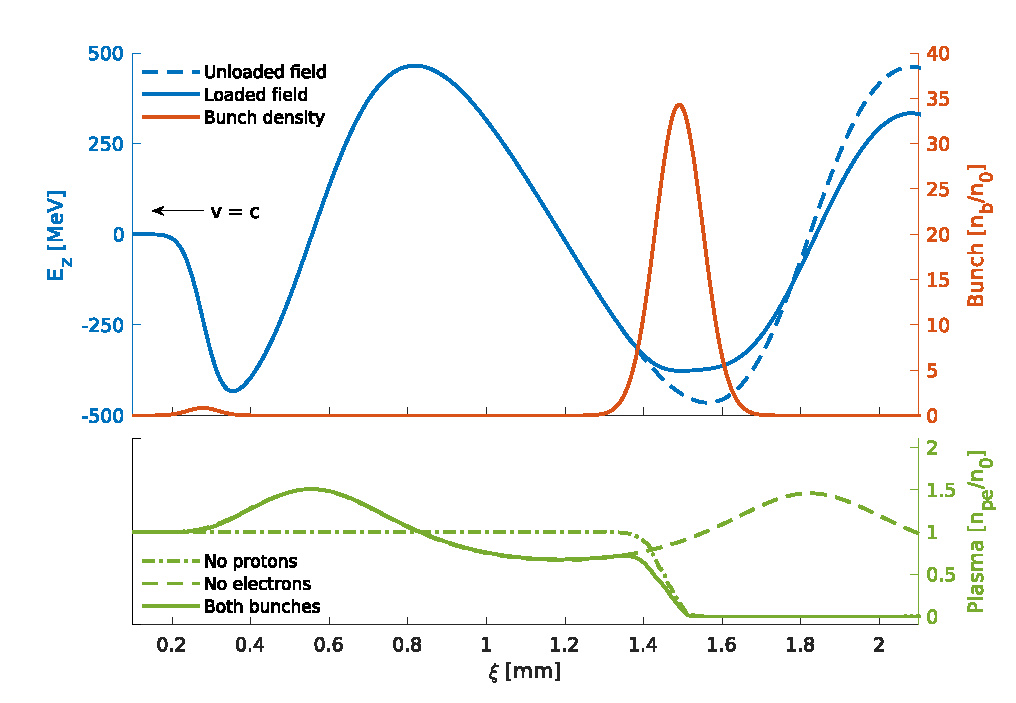
\includegraphics[width=0.8125\linewidth,trim={0mm 0mm 0mm 0mm},clip]{figures/BeamLoading}
    \caption{\label{Fig:BPI:BLoad}
        Example of beam loading of an electron witness bunch on the longitudinal field.
        The bunch density is shown in red, with the (wide) lower density proton drive bunch to the left and the (narrow) high density electron witness bunch to the right.
        The longitudinal wakefield driven by the proton bunch is shown in blue, with the loaded field shown with a solid line and the unloaded field with a dashed line.
        Below, in green, is the corresponding plasma density for only the witness bunch with dash-dotted line, only the proton bunch with dashed line, and both bunches shown with a solid line.
        The figure is recreated from Publication~\ref{Pub:BL17}.
    }
\end{figure}

In the linear case, the challenge is to create a uniform accelerating field in both the transverse and longitudinal direction.
The non-uniformity challenges have been outlined, and solutions proposed for the case of plasma wakefield accelerators, by Van der Meer~\cite{van_der_meer:1985} as well as Katsouleas \etal~\cite{katsouleas:1987} in the 1980s.
The latter suggesting triangular and trapezoidal witness bunches in order to exactly cancel the variations in the field within the bunch.

In the non-linear case, the radial accelerating field variation $W_{z}(r)$ vanishes, provided witness bunch transverse size is within about $2\sigma_{r}$ of the drive bunch~\cite{rosenzweig:1991}.
The longitudinal variation, however, remains.

A short bunch with respect to the accelerating phase of the wakefield, $L \leq \lambda_{pe}/4$, will affect the shape of the plasma electron sheath, but still allows the electrons to return to the axis, while decreasing their transverse momentum.
If the total momentum reaches zero, the witness bunch has extracted all the energy of the accelerating field~\cite{lu:2006a,lu:2006}.
As outlined by Tzoufras \etal~\cite{tzoufras:2009}, a trapezoidal witness bunch with a density maximum at its head can theoretically both flatten the field and achieve a high transformer ratio.
They further show that a flat top bunch is similarly efficient, and Gaussian bunches also have comparable properties -- all being sensitive to fine tuning of position within the bubble, as well as its spot size.

Tzoufras \etal ~provide a solution for the energy absorbed per unit length for an ideal trapezoidal bunch. stating that
\begin{equation}
    Q_{tr}E_{t} = \frac{\pi R_{b}^{4}}{16}, \label{EQ:Trapez}
\end{equation}
where $Q_{tr}$ is the total charge of the trapezoidal bunch, $E_{t}$ is the longitudinal field at the head of the bunch, and $R_{b}$ is the radius of the bubble.
It immediately follows that at optimal beam loading, there is a trade-off between charge and the accelerating gradient and thus energy gain~\cite{tzoufras:2009}.

An example of the longitudinal wakefield loaded by a Gaussian witness bunch, versus the unloaded field, is illustrated in Figure~\ref{Fig:BPI:BLoad}.
The figure is using simulation data from Publication~\ref{Pub:BL17}.

% ================================================================================================================================ %
\subsection{Beam Matching}
\label{Int:BPI:Match}

In the non-linear case, where an ion column is formed, the focusing force it produces will cause a pinching effect on the bunch.
While the bunch itself, assuming the normalised emittance $\emitN > 0$, will naturally expand, there exists a bunch radius where the focusing force and the bunch's tendency to expand are in equilibrium.
For a highly relativistic bunch, $\gammar \gg 1$, the equilibrium radius is given by~\cite{krall:1995}
\begin{equation}
    \sigma_{r,\mathrm{eq}} = \left(2\frac{\emitN^2}{\gammar} \frac{c^2}{\omega_{p}^2} \right)^{1/4}, \label{EQ:BMatch}
\end{equation}
using the emittance definition of Lee and Cooper~\cite{lee:1976}.

This follows from the general envelope equation defined by Lee and Cooper~\cite{lee:1976} under the assumption that: the bunch enters the plasma at focus (i.e. $\deriv\sigma_{r}/\deriv z = 0$), does not diverge significantly from a Gaussian transverse density profile, and that the focusing force is linear~\cite{krall:1995}.

\begin{figure}[hbt]
    \centering
    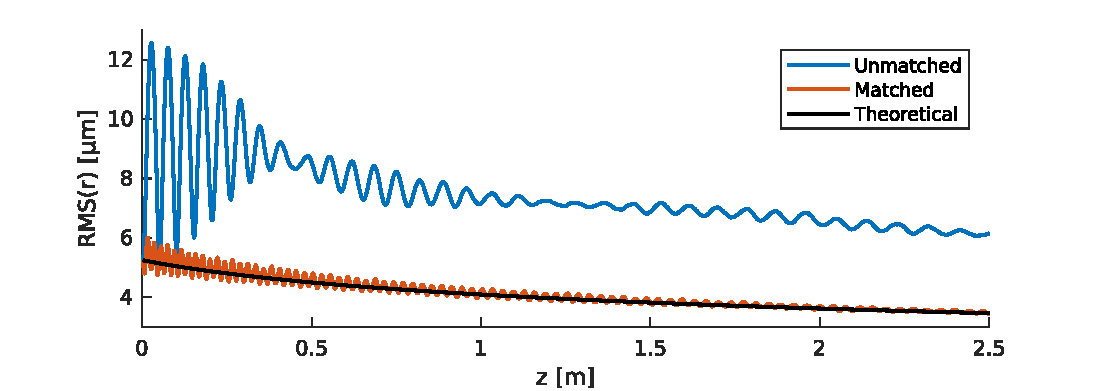
\includegraphics[width=0.875\linewidth,trim={0mm 0mm 0mm 0mm},clip]{figures/BeamMatching}
    \caption{\label{Fig:BPI:Match}
        The evolution of the transverse RMS size of an initially matched electron bunch as it accelerates through a plasma.
        The tail of the bunch, in red, remains in a region where it is matched, while the head of the bunch, in blue, does not.
        The black line corresponds to the theoretical spot size of the bunch at nominal plasma density.
        Based on simulation data from Publication~\ref{Pub:BL17}.
    }
\end{figure}

The simulation in Figure~\ref{Fig:BPI:Match} shows the evolution of the transverse RMS size of an electron bunch as it travels through a plasma.
The bunch has a normalised emittance of $2\unit{\mu m}$, and is initially matched to a plasma density of $7\nexp{14}\unit{cm}^{-3}$ with a $\sigma_{r} = 5.24\unit{\mu m}$.
The tail of the bunch, in red, is in the plasma bubble and thus sees an ion density equal to the plasma density.
The head of the bunch, in blue, where the bubble is forming, sees a lower density.
It is thus not matched, and instead oscillates around an equilibrium point at a larger radius.
The black line is the predicted $\sigma_{r}$ given by Equation~\ref{EQ:BMatch} at initial plasma density, and bunch energy as a function of $z$ as it is accelerated~\cite{berglyd_olsen:2018}.

% ================================================================================================================================ %
\subsection{Multiple Drive Bunches}
\label{Int:BPI:Multi}

As discussed above, larger wakefields can be achieved with multiple drive bunches with a $\lambda_{pe}$ separation.
This happens because such a train of bunches will resonantly drive increasing wakefields.

As outlined by Kallos \etal~\cite{kallos:2007}, when the bunches are longitudinally square, the wakefields scale linearly with the number of bunches.
The shape is of less importance when the bunch length is much less than $\lambda_{pe}$.
However, this does not result in high efficiency as every trailing bunch will see the decelerating field of the earlier bunches.
Efficiency is instead increased when each bunch experience a similar wake field.

This effect can be mitigated in two ways that will in turn maximise transformer ratio.
The first option, named \textit{Ramped Bunch Train}, is to position the bunches with a $1.5\cdot\lambda_{pe}$ separation, such that each bunch is in the accelerating phase of the forward bunches, while at the same time ramp their charge such that the wakefield inside each bunch matches the decelerating field from the first bunch.
This scheme has been demonstrated experimentally by Jing \etal in a dielectric accelerator~\cite{jing:2006,jing:2007}.

The second method described by Kallos \etal, called \textit{Phased Bunch Train}, proposes using short, $k_{pe}l_{z} \ll 1$, equally charged bunches placed in a specific decelerating phase.
The bunch separation needs to be tuned so that the fields inside each bunch matches that of the first bunch.
The phase shift $\theta_{M}$ for the $M$-th bunch is described by Ruth \etal~\cite{ruth:1985}:
\begin{equation}
    \theta_{M} = \sum^{M}_{n=2}\tan^{-1}\left(\frac{1}{\sqrt{n-2}}\right),\quad M \geq 2. \label{EQ:TrainPhase}
\end{equation}
This yields a maximum energy gain
\begin{equation}
    \Delta E_{w} = E_{d,1}\left(2\sqrt{M}-\frac{N_{w}}{N_{d,1}}\right), \label{EQ:TrainPhaseMaxE}
\end{equation}
where $N_{d,1}$ is the first of $M$ drive bunches.
Compared to Eq.~\ref{EQ:TRat:DeltaE} this is an improvement, although not linearly increasing with the number of bunches~\cite{ruth:1985}.

% ================================================================================================================================ %
\section{Using a Proton Drive Beam}
\label{Int:DBeam}

Electron bunches used in previous experiments have a low energy and thus a limited propagation length in the plasma, as can be estimated using Equation~\ref{EQ:Trat:LStop}.

One experiment, at the Stanford Linear Accelerator Center (SLAC)~\cite{blumenfeld:2007}, achieved up to a doubling of energy of electrons with a $42\unit{GeV}$ driver with $1.8\nexp{10}$ particles, corresponding to a total bunch energy of $120\unit{J}$.
The propagation length of such a bunch is on the order of a metre, and the experiment used an $85\unit{cm}$ lithium plasma cell to achieve the energy doubling, with a gradient of up to $52\unit{GeV}$.
Such short accelerator segments are suitable for multi staged accelerators, but they require multiple high energy electron drive bunches. 

% ================================================================================================================================ %
\subsection{Protons vs. Electrons as Drive Beam}
\label{Int:DBeam:PDPWFA}

As ultra-high energy electron bunches are not readily available, the possibility of using proton bunches as driver instead has been of interest for some time~\cite{blue:2003,caldwell:2009}.
The much higher mass carries orders of magnitude more energy at relatively low gamma values.
This effectively eliminates the problem with short propagation lengths in plasma as it scales linearly with the bunch energy; see Equation~\ref{EQ:Trat:LStop}.
Several accelerators exist which delivers kJ-scale proton bunches.
See Table~\ref{T:ProtonBeams} for an overview.

\begin{table}[hbt]
    \centering
    \caption{
        Accelerators world wide with proton bunches with an energy higher than $10\unit{GeV}$.
        The table was compiled by Adli and Muggli~\cite{adli:2016b}, and updated to include the planned upgrade to the LHC.
    }
    \label{T:ProtonBeams}
    \begin{tabularx}{\textwidth}{X R{13mm} R{13mm} R{13mm} R{13mm}}
        \rowcolor{tblhead}
        \texthh{Accelerator} & \multicolumn{2}{c}{\texthh{Max Energy}} & \multicolumn{2}{c}{\texthh{Bunch Length}} \\
        \rowcolor{tblunit}   & \textun{GeV}  & \textun{J}  & \textun{ps}  & \textun{mm} \\
        \hline
        CERN PS, Geneva, Switzerland \cite{assmann:2009}                     &     $26$ &      $540$ &  $1\,000$ &    $300$ \\
        J-PARC, Ibaraki Prefecture, Japan \cite{hotchi:2012}                 &     $30$ & $130\,000$ & $15\,000$ & $4\,500$ \\
        IHEP U70, Protvino, Russia \cite{ivanov:2014}                        &     $50$ &   $4\,000$ & $12\,000$ & $3\,600$ \\
        Fermilab Main Injector, Batavia, Illinois, USA \cite{nagaitsev:2014} &    $120$ &   $2\,100$ &     $600$ &    $180$ \\
        CERN SPS, Geneva, Switzerland \cite{assmann:2009}                    &    $450$ &   $8\,300$ &     $400$ &    $120$ \\
        CERN LHC, Geneva, Switzerland \cite{assmann:2009}                    & $7\,000$ & $124\,000$ &     $250$ &     $75$ \\
        CERN HL-LHC, Geneva, Switzerland \cite{apollinari:2017}              & $7\,000$ & $247\,000$ &     $270$ &     $81$ \\
        \hline
    \end{tabularx}
\end{table}

However, in order to produce GV/m-scale plasma wakefield accelerators, the plasma density needs to be $\gtrsim 10^{14}\unit{cm}^{-3}$; see Equation~\ref{EQ:EWB}.
This corresponds to plasma wavelengths on the order of a few millimetres.
To maximise efficiency in the transfer of energy from the drive bunch to the plasma, as discussed in Section~\ref{Int:BPI:TRat}, the bunch must satisfy $k_{pe}\sigma_{z} \simeq \sqrt{2}$.
Such short bunches are not readily available, but options for creating short bunches have been proposed~\cite{assmann:2009}.
On the other hand, the problem with $\gg\lambda_{pe}$ proton bunches can be solved by exploiting one of several instabilities that can occur when a long bunch propagates through plasma.

% ================================================================================================================================ %
\subsection{The Self-Modulation Instability}
\label{Int:DBeam:SMI}

A long bunch with respect to the plasma wavelength will generate a density wave driven by its own head.
This is true for both laser beams~\cite{esarey:1994} and particle bunches~\cite{kumar:2010}, and they are caused by the same underlying physics.
For a laser beam, the self-modulation arises from alternating regions of focusing and diffraction.
For a particle bunch, the wakefields generated within the bunch acts back on itself, breaking it up into short micro bunches with a surrounding, defocused halo.

In the 1980s this self-modulating effect was taken advantage of in LWFA experiments as only long laser pulses were available.
Advances in ultra short laser technology later removed the dependence of this effect~\cite{pukhov:2002}, but for proton bunches, this remains a challenge.
However, the self-modulation instability can also be exploited for proton bunches to generate high accelerating gradients~\cite{schroeder:2012,schroeder:2011,caldwell:2009}.

Beam self-modulation is caused by a transverse two-stream instability which occurs for a bunch with a radius on the order of the plasma skin depth, $\sigma_{r} \simeq c/\omega_{pe}$~\cite{vieira:2012}.
Much narrower bunches will see pinching effects, while wider bunches will experience to filamentation instabilities~\cite{keinigs:1987}.

The micro bunching caused by self-modulation has a period close to the plasma wavelength, but long bunches are also subject to hosing instabilities~\cite{whittum:1991}, an effect also seen in long laser beams~\cite{duda:1999,duda:2000}.
This may prove to be a limitation to stability over long propagation lengths.
Hosing, however, can be prevented by the breaking up of the bunch caused by self-modulation \cite{vieira:2014}.
A sharp leading edge of the bunch can be used to seed modulation \cite{fang:2014}.
Seeding can significantly reduce the risk of hosing.
This is also the case for long laser pulses, and resolved by seeding~\cite{vieira:2012}. 

Self-modulation has been shown experimentally for long electron bunches at SLAC~\cite{muggli:2014,muggli:2015} as well halo formation on short and long positron bunches~\cite{muggli:2008,hogan:2003}.
Self-modulation has also recently been seen for proton bunches at AWAKE~\cite{muggli:2017a}.

% ================================================================================================================================ %
